

\chapter{Þyngdarlögmálið}

\section{Þyngdarlögmál Newtons}

\begin{tcolorbox}
\begin{definition}
Lítum á tvo massa, $m_1$ og $m_2$ sem eru í fjarlægð $r$ frá hvor öðrum. Þá verkar á milli þeirra aðdráttarkraftur, $F_G$, sem kallast \textbf{þyngdarlögmálskrafturinn} og er gefinn með:
\begin{align*}
    F_G = G \frac{m_1 m_2}{r^2},
\end{align*}
þar sem $G = \SI{6.67e-11}{m^3/(kg.s^2)}$ er fasti sem nefnist \textbf{þyngdarlögmálsfastinn}.
\end{definition}
\end{tcolorbox}

\begin{figure}[H]
    \centering
    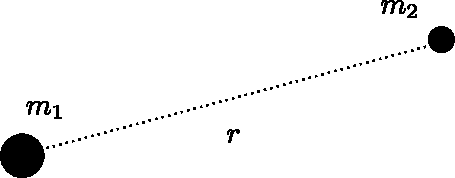
\includegraphics[scale = 0.75]{figures/fG.pdf}
    \caption{Tveir massar, $m_1$ og $m_2$ í fjarlægð $r$ frá hvor öðrum.}
\end{figure}


Þetta er útvíkkun á þyngdarkraftinum, $F_g$, sem við höfum þegar kynnst. Þannig við vitum að á yfirborði jarðarinnar þá þurfa þyngdarkrafturinn og þyngdarlögmálskrafturinn að vera sammála, þ.e. við höfum að $F_g = F_G$ á yfirborði jarðinnar en það þýðir að ef massi okkar er $m$, massi jarðarinnar er $M$ og geisli jarðarinnar er $R$, þá gildir að:
\begin{align*}
    F_g = F_G \implies mg = \frac{GmM}{R^2} \implies g = \frac{GM}{R^2}
\end{align*}
\begin{tcolorbox}
\begin{theorem}
Þyngdarlögmálskrafturinn er geyminn. Stöðuorka massans $m$ í fjarlægð $r_0$ frá $M$ miðað við viðmiðunarpunktinn $r = +\infty$ er gefin með:
\begin{align*}
    U_G = -\frac{GM m}{r_0}.
\end{align*}
\end{theorem}
\end{tcolorbox}

\textbf{Útleiðsla:} Við setjum viðmiðunarpunkt stöðuorkunnar í $r = \infty$. Þar er þyngdarlögmálskrafturinn sem verkar á hlutinn gefinn með $F_G = 0$. Við viljum síðan reikna vinnuna sem að hlutur þarf að vinna til þess að fara frá $r = \infty$ í $r = r_0$. Við fáum því:
\begin{align*}
    U_G = -W_G = - \int_{+\infty}^{r_0} -\frac{GMm}{r^2} dr = -\left[  \frac{GMm}{r} \right]_{+\infty}^{r_0} = -\frac{GMm}{r_0}.
\end{align*}
\qed

\begin{comment}
\begin{tcolorbox}
\begin{theorem}
Þyngdarfastinn, $g$ og þyngdarlögmálsfastinn, $G$, tengjast með eftirfarandi hætti:
\begin{align*}
    g = \frac{GM}{R^2}.
\end{align*}
\end{theorem}
\end{tcolorbox}
\end{comment}

\begin{comment}
\textbf{Útleiðsla:} Við vitum að á yfirborði jarðarinnar eru þyngdarlögmálskrafturinn og þyngdarkrafturinn sami krafturinn þannig að við höfum að:
\begin{align*}
    mg = \frac{GMm}{R^2} \implies g = \frac{GM}{R^2}.
\end{align*}
\end{comment}



\section{Hringhreyfing}

\begin{minipage}{\linewidth}
\begin{wrapfigure}{r}{2.8in}
\vspace{-1cm}
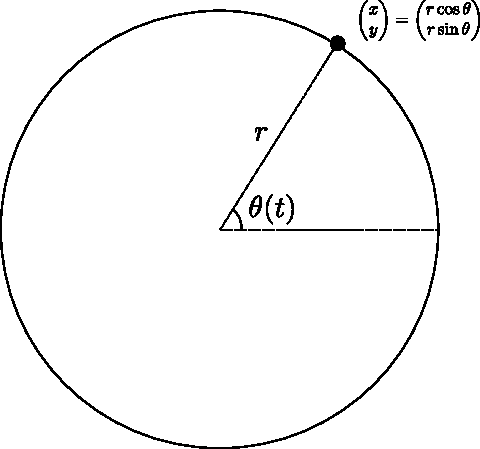
\includegraphics[width=3in]{figures/hringhreyfing2.pdf}
\caption{Hlutur á hringhreyfingu.}
\label{fig:fnun}
\end{wrapfigure}

Skoðum núna hlut sem er á hringhreyfingu með geisla $r$ og hraða $v$. Við getum þá skrifað staðsetningu hlutarins sem fall af tíma sem:
\begin{align*}
    \vec{r}(t) = \begin{pmatrix} x(t) \\ y(t) \end{pmatrix} = \begin{pmatrix} r\cos\theta(t) \\ r\sin\theta(t) \end{pmatrix},
\end{align*}
þar sem að $r = \abs{\vec{r}(t)}$ er geisli hringsins og $\theta(t)$ er hornið sem lýsir staðsetningu hlutarins sem fall af tíma $t$. Jörðin fer einn hring á einu ári svo að við vitum að heildarvegalengdin sem hún þarf að ferðast á einu ári, $T = \SI{1}{ár}$, er gefin með $s = 2\pi r$, þar sem $r = \SI{1}{AU} = \SI{1.5e11}{m}$, er vegalengdin milli jarðarinnar og sólarinnar. Við vitum þá að hraðinn sem að jörðin þarf að ferðast með er gefin með:
\begin{align*}
    v = \frac{s}{T} = \frac{2\pi r}{T} = \frac{2 \pi \cdot \SI{1.5e11}{m}}{365 \cdot 24 \cdot 60^2} = \SI{30}{km/s}.
\end{align*}
Við viljum skilja hvernig að hornið breytist sem fall af tíma $t$. Við athugum að ef $t$ táknar tímann sem hefur liðið frá því að árið byrjaði þá er $\frac{t}{T}$ hlutfallið sem að við höfum farið meðfram hringnum það árið. En við vitum að hringurinn er $\ang{360}$ eða í radíönum $2\pi$ og því höfum við að:
\end{minipage}

\begin{align*}
    \frac{t}{T} = \frac{\theta}{2\pi} \implies \theta = \frac{2\pi t}{T}
\end{align*}
En við vitum að $v = \frac{2\pi r}{T}$ svo $T = \frac{2\pi r}{v}$ sem gefur okkur því að:
\begin{align*}
    \theta = \frac{2\pi t}{T} = \frac{2\pi t}{\frac{2\pi r}{v}} = \frac{v}{r}t.
\end{align*}
Á þessum tímapunkti er eðlilegt að kynna stærð sem kallast hornhraði og er táknuð með $\omega$ og er skilgreind þannig að
\begin{align*}
    \omega = \frac{d\theta}{dt}.
\end{align*}
Til samanburðar er hraði skilgreindur þannig að $v = \frac{ds}{dt}$. Fyrir hringhreyfingu þá er hornhraði hlutarins fastur og við höfum einmitt að hornhraði jarðarinnar á hringferð sinni um sólina er gefinn með:
\begin{align*}
    \omega = \frac{2\pi}{T} = \frac{2\pi}{(365 \cdot 24 \cdot 60^2 \, \si{s})} = \SI{2.0e-7}{rad/s}
\end{align*}
Þar sem að á einu ári þá fer hornið $\theta$ frá því að vera $\SI{0}{rad}$ í það að vera $2\pi \si{rad}$. Eins og sjá má hér að ofan eru SI-einingar hornhraða gefnar með $\si{rad/s}$. En þar sem að hornhraðinn er fastur þá gildir að:
\begin{align*}
    \omega = \frac{\theta}{t} \implies \theta = \omega t
\end{align*}
En við höfum áður sýnt að:
\begin{align*}
    \theta = \frac{v}{r}t
\end{align*}
Svo við ályktum að fyrir hlut á hringhreyfingu gildir að hraði hlutarins og hornhraðinn tengjast með eftirfarandi hætti:
\begin{align*}
    \omega = \frac{v}{r}
\end{align*}

Þetta er oftast skrifað línulega sem:
\begin{align*}
    v  = r\omega.
\end{align*}
Fyrir jörðina höfum við sýnt að $v = \SI{30}{km/s}$. En við höfum einmitt að:
\begin{align*}
    \omega r = \SI{2.0e-7}{rad/s} \cdot \SI{1.5e11}{m} = \SI{30}{km/s},
\end{align*}
eins og við var að búast. Við höfum semsagt sýnt að stöðuvigur hlutar á hringhreyfingu er gefinn með:
\begin{align*}
    \vec{r} = \begin{pmatrix} r\cos\theta \\ r\sin\theta \end{pmatrix}
\end{align*}

og við vitum að hraði hlutarins er hornréttur á stöðuvigurinn, réttara sagt er hann þvervigur stöðuvigursins (sem hefur aðra lengd). En það þýðir að:
\begin{align*}
    \vec{v} = \begin{pmatrix} -v \sin\theta \\ v \cos\theta \end{pmatrix}
\end{align*}
En við vitum að $v = \frac{2\pi r}{T} = \omega r$ svo við höfum að:
\begin{align*}
    \vec{v} = \begin{pmatrix} -\omega r \sin\theta \\ \omega r \cos\theta \end{pmatrix} = \omega \hat{\vec{r}}.
\end{align*}
Þar sem að $\hat{\vec{r}}$ táknar þvervigur vigursins $\vec{r}$, þ.e.
\begin{align*}
    \hat{\vec{r}} = \begin{pmatrix} -r \sin\theta \\ r \cos\theta \end{pmatrix}.
\end{align*}
Við sjáum þá að lengd vigursins breytist bara þannig að hún margfaldast með $\omega$. Við vitum að lokum að hröðun hlutarins er inn að miðju hringsins (þar sem að eini krafturinn sem verkar á jörðina er þyngdarlögmálskrafturinn milli jarðarinnar og sólarinnar). En þar með fáum við að lokum að:
\begin{align*}
    \vec{a} = \omega^2 \hat{\hat{\vec{r}}} = -\omega^2 \vec{r}.
\end{align*}
Þar sem að við sjáum að $\vec{a}$ og $\vec{r}$ eru gagnstefna. En þar með höfum við að stærð vigursins $\vec{a}$ er gefin með:
\begin{align*}
    a = \abs{\vec{a}} = \omega^2 r = \left(\frac{v}{r}\right)^2 r = \frac{v^2}{r}.
\end{align*}
Við höfum því sýnt að hröðun hlutar á hringhreyfingu er inn að miðju hringsins og er gefin með $a = \frac{v^2}{r}$. Þessi hröðun kallast miðsóknarhröðun hlutarins og við köllum kraftinn sem að veldur hröðuninni miðsóknarkraft. En við getum líka skrifað hröðunina á annan veg með því að rifja upp að $v = \frac{2\pi r}{T}$ svo við höfum að:
\begin{align*}
    a = \frac{v^2}{r} = \frac{\left( \frac{2\pi r}{T} \right)^2}{r} = \frac{4\pi^2 r}{T^2}.
\end{align*}
Við getum einnig leitt þetta út með víddargreiningu. Þá athugum við að:
\begin{align*}
    a = m^{\alpha}v^\beta r^\gamma
\end{align*}
og með því að skoða víddirnar á stærðunum þá höfum við að:
\begin{align*}
    \left[ a \right] = [m]^{\alpha}[v]^\beta [r]^\gamma \implies \si[per-mode=fraction]{\frac{m}{s^2}} = \si{kg}^\alpha \left(\si{\frac{m}{s}}\right)^\beta \si{m}^\gamma \implies \si{kg}^{0}\si{m}^1 \si{s}^{-2} = \si{kg}^\alpha \si{m}^{\beta + \gamma} \si{s}^{-\beta}
\end{align*}
Sem gefur okkur eftirfarandi jöfnuhneppi:
\begin{align*}
    \begin{cases}
    \alpha = 0 \\
    \beta + \gamma = 1 \\
    -\beta = -2
    \end{cases}
\end{align*}
En það jöfnuhneppi hefur lausnina $(\alpha, \beta, \gamma) = (0,2,-1)$ sem þýðir að:
\begin{align*}
    a = m^{\alpha}v^\beta r^\gamma = v^2r^{-1} = \frac{v^2}{r}.
\end{align*}
Fyrir hlut á hringhreyfingu.



\section{Þriðja lögmál Keplers fyrir hringhreyfingu}

\begin{minipage}{\linewidth}
\begin{wrapfigure}{r}{2.3in}
\vspace{-1cm}
\centering
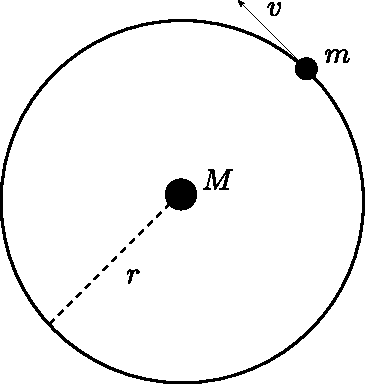
\includegraphics[width=2in]{figures/planets.pdf}
\caption{Lítill massi, $m$, með hraða $v$ á hringhreyfingu með geisla $r$ um stóran massa $M$.}
\label{fig:hringhreyfing}
\end{wrapfigure}

Við skulum nú skoða hlut með lítinn massa, $m$, sem hefur hraðann $v$ og er á hringhreyfingu með geisla $r$ um stóran massa, $M$. Við hugsum okkur til að byrja með að litli massinn, $m$, tákni jörðina og stóri massinn, $M$, tákni sólina. En það kemur í ljós að lögmálið gildir engu að síður fyrir hvaða hringhreyfingu (með föstum hraða) sem er. Þannig gildir lögmálið eins fyrir tungl á hringferð umhverfis reikistjörnu. Við höfum samkvæmt þyngdarlögmálinu að krafturinn sem verkar á pláneturnar vegna sólarinnar er gefinn með:
\begin{align*}
    F_G = \frac{GMm}{r^2}.
\end{align*}
En þar sem að þetta er eini krafturinn sem að verkar á plánetuna sem er á hringhreyfingu um sólina þá höfum við samkvæmt öðru lögmáli Newtons að:
\end{minipage}
\begin{align*}
    F_{\text{heild}} = F_G,
\end{align*}
og þar sem að plánetan er á hringhreyfingu höfum við að:
\begin{align*}
    ma = m \frac{v^2}{r} = \frac{GMm}{r^2}
\end{align*}
En með því að stytta út $m$ og margfalda í gegn með $r$ höfum við því að:
\begin{align*}
    v^2 = \frac{GM}{r}.
\end{align*}
En nú ferðast plánetan með jöfnum hraða umhverfis sólina svo við höfum að hraði hennar er gefinn með:
\begin{align*}
    v = \frac{2\pi r}{T}.
\end{align*}
En þar með getum við ályktað að:
\begin{align*}
    \frac{GM}{r} = v^2 =  \left( \frac{2\pi r}{T} \right)^2 = \frac{4\pi^2r^2}{T^2}
\end{align*}
En þetta getum við umritað sem:
\begin{align*}
    \frac{r^3}{T^2} = \frac{GM}{4\pi^2} = \text{fasti}.
\end{align*}
Við höfum því sýnt:

\begin{tcolorbox}
\begin{theorem}
    \textbf{(Þriðja lögmál Keplers)} Lítum á lítinn massa $m$ með hraða $v$ sem er á hringhreyfingu með geisla $r$ um stórann massa $M$. Látum $T$ vera umferðartíma massans $m$ um stóra massann $M$. Þá gildir að:
\begin{align*}
    \frac{r^3}{T^2} = \frac{GM}{4\pi^2} = \text{fasti}.
\end{align*}
\end{theorem}
\end{tcolorbox}

Við notum þetta lögmál oft með eftirfarandi hætti. Hugsum okkur að við séum með tvær plánetur (t.d. jörðina og Venusi) sem eru á hringhreyfingu með geisla $r_1$ og $r_2$ hvor um sig frá sólinni og hafa umferðartíma $T_1$ og $T_2$ umhverfis sólina. Við höfum þá að:
\begin{align*}
    \frac{r_1^3}{T_1^2} = \frac{GM}{4\pi^2} = \frac{r_2^3}{T_2^2} \implies \frac{a_1^3}{T_1^2} = \frac{a_2^3}{T_2^2}.
\end{align*}







\newpage

\section{Lögmál Keplers}


Johannes Kepler setti fram lögmál um hreyfingu himinhnattanna á árunum 1609-1619. Það var síðan Isaaq Newton sem leiddi þau út og sýndi að þau væru í samræmi við þyngdarlögmálið hans árið 1687 í öndvegisriti sínu, Principia. Við gerðum í síðustu grein ráð fyrir því að pláneturnar ferðist með jöfnum hraða á hring umhverfis sólina. Það er ekki alveg rétt, því í rauninni ferðast þær á sporbaug (sem er eins og egglaga hringur) en það er afskaplega góð nálgun að þær séu á hringhreyfingu því það kemur í ljós að miðvik sporbauganna sem pláneturnar ferðast eftir er svo lítið að þær eru svo gott sem á hringhreyfingu. Við byrjum á því að skilgreina hvað við meinum með sporbaug:

\begin{tcolorbox}
\begin{definition}
\textbf{Sporbaugur} (eða ellipsa) er safn þeirra punkta sem uppfylla jöfnuna:
\begin{align*}
    \frac{x^2}{a^2} + \frac{y^2}{b^2} = 1.
\end{align*}
Talan $a$ kallast þá \textbf{langás} sporbaugsins en talan $b$ kallast \textbf{skammás} sporbaugsins. Við skilgreinum \textbf{brennipunkta} ellipsunnar sem punktana $F_1 = (-c,0)$ og $F_2 = (c,0)$ þar sem $c =\sqrt{a^2 - b^2}$. Við skilgreinum \textbf{miðvik} sporbaugsins sem stærðina $ \varepsilon = \frac{c}{a}$.
\end{definition}
\end{tcolorbox}

Við tökum eftir að þegar $a = b = r$ þá fáum við hring, því þá höfum við $\frac{x^2}{r^2}+ \frac{y^2}{r^2} = 1$ eða með því að margfalda í gegn með $r^2$ þá sjáum við að við höfum $x^2 + y^2 = r^2$ sem er jafna hrings. Sporbaugurinn er því í einhverjum skilningi útvíkkun á hugtakinu sem við þekkjum nú þegar fyrir hring. Við tökum líka eftir því að miðvik sporbaugsins, $\varepsilon$ getur mest orðið $\varepsilon = \frac{a}{a} = 1$ en það gerist þegar $b = 0$ (þegar ellipsan verður að línu). Við sjáum einnig að miðvik sporbaugsins, $\varepsilon$, getur minnst orðið $\varepsilon = \frac{0}{a} = 0$, en það gerist þegar $b = a$ eða þegar ellipsan samsvarar hring. Þannig $\varepsilon \in [0,1]$ og $\varepsilon = 0$ samsvarar hring en $\varepsilon = 1$ samsvarar línu. 

\begin{figure}[H]
    \centering
\begin{subfigure}[h]{.4\textwidth}
    \centering
    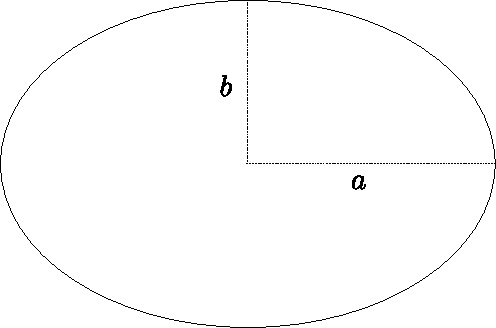
\includegraphics[width=\linewidth]{figures/ellipse1.pdf}
    \caption{Sporbaugur með langás $a$ og skammás $b$.}
    \label{fig:ellipse}
\end{subfigure}
\hfill
\begin{subfigure}[h]{.4\textwidth}
    \centering
    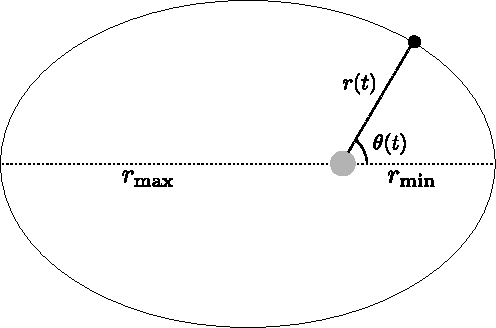
\includegraphics[width=\linewidth]{figures/keplerfirstlaw}
    \caption{Pláneturnar ferðast á sporbaug í kringum sólina með sólina í öðrum brennipunktinum.}
    \label{subfig:FirstKepler}
\end{subfigure}
\end{figure}


\subsection*{Fyrsta lögmál Keplers}

\begin{tcolorbox}
\begin{theorem}
Pláneturnar ferðast á sporbaug í kringum sólina með sólina í öðrum brennipunktinum.
\end{theorem}
\end{tcolorbox}

\begin{comment}
Þá má lýsa fjarlægð reikistjarnanna frá sólinni með:
\begin{align*}
    r(t) = \frac{a(1-\varepsilon^2)}{1- \varepsilon \cos\theta(t)}
\end{align*}
\end{theorem}
Þar sem $a$ og $\varepsilon$ eru langás og miðvik sporbaugsins og $\theta(t)$ er hornið sem sólin og reikistjarnan sveipa.
\end{comment}

Við sjáum þá að:
\begin{align*}
    a = \frac{r_{\text{max}}+ r_{\text{min}}}{2}.
\end{align*}


Fyrir jörðin þá höfum við að mesta fjarlægðin milli jarðarinnar og sólarinnar er gefin með $r_{\text{max}} = \SI{1.521e11}{m}$ en minnsta fjarlægðin er gefin með $r_{\text{min}} = \SI{1.471e11}{m}$. Við höfum þá að langás sporbaugsins sem jörðin ferðast eftir er gefinn með $a_{_{J}} = \frac{1}{2}(r_{\text{max}} + r_{\text{min}}) = \SI{1.496e11}{m}$. Við tökum síðan eftir því að $r_{\text{max}} = a + c$ en þá er $c_{_{J}} = r_{\text{max}} - a_{_{J}} = \SI{0.025e11}{m}$. Það þýðir að miðvik sporbaugsins sem jörðin ferðast í kringum sólina með er $\varepsilon_{_{J}} = \frac{c_{_{J}}}{a_{_{J}}} = \frac{\SI{0.025e11}{m}}{\SI{1.496e11}{m}} = 0.01671$.
Sem þýðir að $\varepsilon_{_J} \approx 0$ og það er því góð nálgun að gera ráð fyrir að jörðin sé á hringhreyfingu um sólina.

\subsection*{Annað lögmál Keplers}

\begin{tcolorbox}
\begin{theorem}
Línan frá sólu að reikistjörnu fer á hverju tímabili yfir jafnstórt flatarmál.
\end{theorem}
\end{tcolorbox}

\begin{figure}[H]
    \centering
    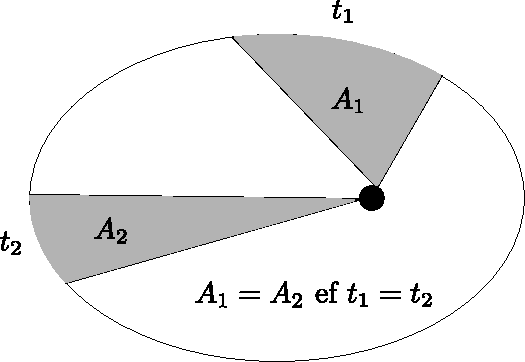
\includegraphics[scale = 0.8]{figures/keplersecondlaw.pdf}
    \caption{Flatarmálið, $A(t)$, sem pláneturnar sveipa á tíma $t$ er alltaf jafn stórt.}
    \label{fig:kepler2ndlaw}
\end{figure}



\subsection*{Þriðja lögmál Keplers fyrir sporbauga}

\begin{tcolorbox}
\begin{theorem}
    Lítum á lítinn massa, $m$ sem ferðast á sporbaug um stóran massa $M$ sem er staddur í brennipunkti sporbaugsins. Látum $a$ vera langás sporbaugsins og látum $T$ tákna umferðartíma litla massans umhverfis stóra massann. Þá gildir að:
\begin{align*}
    \frac{a^3}{T^2} = \frac{G(M+m)}{4\pi^2} \approx \frac{GM}{4\pi^2} = \text{fasti}.
\end{align*}
\end{theorem}
\end{tcolorbox}


\begin{comment}

\section{Tengsl þyngdarlögmálskraftsins við þyngdarkraftinn}

\begin{tcolorbox}
\begin{definition}
Við segjum að stærð $a$ sé miklu minni en stærð $b$ og skrifum að $a \ll b$ ef að hlutfallið $\frac{a}{b}$ er lítið.
\end{definition}
\end{tcolorbox}

\begin{tcolorbox}
\begin{setning}
Látum $b \ll 1$
\end{setning}
\end{tcolorbox}

\textbf{Sönnun:} Við athugum að:
\begin{align*}
    (1+b)^n = 1 + nb + \frac{n(n-1)}{2}b^2 + \ldots + b^n
\end{align*}
Þar sem $b \ll 1$ þá getum við sleppt öllum liðum sem eru stærri en $b^2$. Við skrifum þá stundum að:
\begin{align*}
    (1+b)^n = 1 + nb + \mathcal{O}(b^2).
\end{align*}
Til að tákna það að við hunsum alla liði sem eru stærri en $b$ (vegna þess að þeir eru litlir).


\begin{align*}
     \frac{Gm M_J}{(R_J + h)^2} = \frac{GmM_J}{{R_J}^2(1 + \frac{h}{R_J})^2} = \frac{GmM_J}{{R_J}^2}\frac{1}{(1 + \frac{h}{R_J})^2} = mg(1 + \frac{h}{R_J})^{-2} \stackrel{h \ll R_J}{\approx} mg \left(1 - \frac{2h}{R_J} \right)
\end{align*}

\end{comment}

\begin{comment}
\section{Heimsmyndarfræði}

Í þessum kafla ætlum við að skoða heimsmyndarfræði. Sagan okkar hefst eins og margar aðrar góðar sögur hjá Forn-Grikkjum. Sagan segir að Eratosþenes (sem var bókasafnsvörður á bókasafninu í Alexandríu) hafi lesið sér til um að í Síennu við hádegi á sumarsólstöðum væri hægt að líta niður í brunn um hádegi og sjá sólina endurvarpast af vatninu niðri í brunninum. Hann ályktaði því að sólin hlyti að vera beint yfir höfði í Síennu við hádegi á sumarsólstöðum. En þá, ef jörðin væri kúlulaga þá ætti sólin að varpa skugga á jörðina í Alexandríu á sama tíma. Þannig á næstu sumarsólstöðum þá festi Eratosþenes spýtu niður í jörðina hornrétt á yfirborðið í Alexandríu. Við hádegisbil þá mældi hann skuggann sem sólin varpaði á spýtuna og reiknaði þá að hornið sem sólin kæmi niður undir væri um $\SI{7}{\degree}$. Út frá þessu ásamt vegalengdinni milli Alexandríu og Síennu gat Eratosþenes lagt mat á geisla jarðarinnar.

\begin{table}[H]
    \centering
    \begin{tabular}{|c|l|l|}
        \hline
        \textbf{Ár}  & \textbf{Viðburður} & \textbf{Uppgötvun} \\ \hline
        -200  & Geisli jarðarinnar mældur & Eratosþenes \\ \hline
        1619 & Lögmál Keplers & Kepler \\ \hline
        1676 & Ljóshraðinn mældur & Ole Rømer \\ \hline
        1689 & Þyngdarlögmálið & Newton \\ \hline
        1769 & Stjarnfræðieiningin & Edmond Halley \\ \hline
        1797 & Þyngdarlögmálsfastinn mældur & Cavendish \\ \hline
        1797 & Vegalengdin til tunglsins & Cavendish \\ \hline
        1905 & Takmarkaða afstæðiskenningin & Albert Einstein \\ \hline
        1915 & Almenna afstæðiskenningin & Albert Einstein \\ \hline
    \end{tabular}
    \caption{Nokkrir merkilegir viðburðir í vísindasögunni.}
    \label{tafla:saga}
\end{table}
\end{comment}

\section{Sýnidæmi}

\subsection*{Rómeo og Júlía}

Fólk talar stundum um aðdráttarkraft ástarinnar í daglegu tali. Þá tölum við um að fólk laðist að öðru fólki (nefnum engin kyn hérna). Í upphafsatriði bandarísku bíómyndarinnar \duck{Back to the Future} er til dæmis lagið  \duck{The Power of Love} spilað á meðan Marty McFly teikar bíl í skólann á hjólabrettinu sínu. Hugsum okkur því núna að Rómeó og Júlía standi í fjarlægð $r = \SI{8.5}{cm}$ frá hvort örðu (við miðum við fjarlægðina á milli massamiðjunnar á þeim). Látum Rómeó hafa massa $m_R = \SI{67}{kg}$ og Júlíu hafa massa $m_J = \SI{88}{kg}$. Þá er þyngdarlögmálskrafturinn sem verkar á milli þeirra gefinn með:
\begin{align*}
    F_G = \frac{Gm_R m_J}{r^2} = \frac{\SI{6.67e-11}{m^3/(kg.s^2)} \cdot \SI{67}{kg}\cdot\SI{88}{kg}}{(\SI{8.5e-2}{m})^2} = \SI{5.4e-5}{N}.
\end{align*}
Við sjáum þá að aðdráttarkrafturinn sem verkar á milli þeirra er miklu minni heldur en þyngdarkrafturinn sem verkar á þau vegna jarðarinnar, en hann er annarsvegar fyrir Rómeó $m_R g = \SI{660}{N}$ og hinsvegar fyrir Júlíu $m_Jg = \SI{860}{N}$. Sem er bæði miklu stærra heldur en $F_G = \SI{5.4e-5}{N}$. Við sjáum einnig að Rómeó laðast meira að Júlíu (einfaldlega því hún hefur meiri massa en Rómeó). Hröðun Rómeós til Júlíu væri þá gefin með:
\begin{align*}
    m_R a_R = F_G \implies a_R = \frac{F_G}{m_R} = \SI{8.0e-7}{m/s^2}.
\end{align*}
Eins væri hröðunin sem Júlía myndi finna fyrir í áttina að Rómeó gefin með:
\begin{align*}
    m_J a_J = F_G \implies a_J = \frac{F_G}{m_J} = \SI{6.1e-7}{m/s^2} < a_R.
\end{align*}

\newpage

\subsection*{Lagrange-punktar}

Þar sem að þyngdarlögmálskrafturinn er aðdráttarkraftur sem verkar á milli sérhverra tveggja massa þá gefur það til kynna að til sé punktur á milli jarðarinnar og sólarinnar þar sem að heildarkrafturinn sem verkar á hlutinn sé núll. Með öðrum orðum, ef $d = \SI{1.0}{AU} = \SI{1.50e11}{m}$ er fjarlægðin milli jarðarinnar og sólarinnar þá er til fjarlægð $0 < x < d$ frá sólinni þar sem að heildarkrafturinn sem verkar á hlutinn er núll. Slíkir punktar kallast Lagrange-punktar. Við höfum þá að ef $F_S$ táknar þyngdarlögmálskraftinn sem verkar á milli massans, $m$ og sólarinnar og $F_J$ táknar þyngdarlögmálskraftinn sem verkar á milli jarðarinnar og massans, $m$. Þá gildir að:
\begin{align*}
    F_S = F_J \implies \frac{GM_Sm}{x^2} = \frac{GM_Jm}{(d-x)^2} \implies \frac{(d-x)^2}{x^2} = \frac{M_J}{M_S}
\end{align*}
Sem við getum umritað þannig að:
\begin{align*}
    \left( \frac{d}{x}-1 \right)^2 = \frac{M_J}{M_S} \implies \frac{d}{x}-1 =  \pm \sqrt{\frac{M_J}{M_S}}
\end{align*}
Við veljum jákvæða formerkið því $d > x$ svo $\left(\frac{d}{x}-1\right) > 0$. En þar með höfum við að:
\begin{align*}
    \frac{d}{x} = 1 + \sqrt{\frac{M_J}{M_S}} \implies x = \frac{d}{1+\sqrt{\frac{M_J}{M_S}}} = \frac{\SI{1.0}{AU}}{1+ \sqrt{\frac{\SI{2.0e30}{kg}}{\SI{5.97e24}{kg}}}} = \SI{0.998}{AU}.
\end{align*}
Sem er fjarlægðin frá sólinni að Lagrange-punktinum. En sá punktur er þá í fjarlægðinni $d-x = \SI{0.002}{AU}$ frá jörðinni. Þessi punktur er reyndar ekki eini Lagrange-punkturinn sem að jörðin og sólin hafa á milli sín. Þessi punktur er iðulega kallaður $L_1$ þar sem að það eru í heildina fimm punktar í sólkerfinu þar sem að heildkrafturinn sem verkar á hlut í þeim punkti er núll frá jörðinni og sólinni. Nokkrum gervitunglum hefur verið komið fyrir í $L_1$ eins og t.d.~ACE og DSCOVR gervitunglin. Það er hinsvegar erfitt að skýla gervitunglum þar frá miklum og öflugum sólvindum svo slík gervitungl endast ekki lengi.

\subsection*{Að snúa bolta í bandi}

\begin{minipage}{\linewidth}
\begin{wrapfigure}{r}{2.3in}
\vspace{-1cm}
\centering
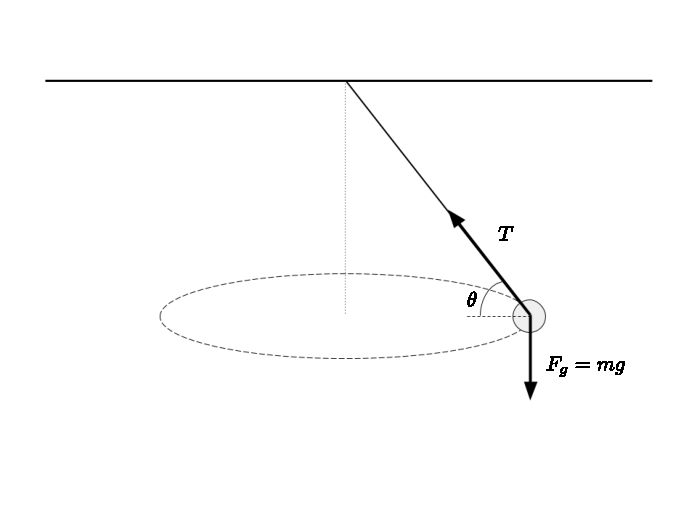
\includegraphics[width=2.5in]{temp/togberthringbert.pdf}
\caption{Bolta með massa $m$ snýst í hringi með jöfnum hraða $v$ á hring með geisla $r$. Lengd bandsins er $\ell$ og hornið sem bandið m.v.~lárétt er $\theta$.}
\label{fig:togkraftshringhreyf}
\end{wrapfigure}

Hugsum okkur að við séum að snúa bolta í bandi í lárétta hringi með hraða $v$. Ef við skrifum niður kraftajöfnu fyrir hlutinn þá höfum við:
\begin{align*}
    \begin{pmatrix} ma \\ 0 \end{pmatrix} = \begin{pmatrix} T\cos\theta \\ T\sin\theta - mg \end{pmatrix}
\end{align*}
En við sjáum þá úr neðri jöfnunni að:
\begin{align*}
    T = \frac{mg}{\sin\theta}.
\end{align*}
En þá gefur efri jafnan að:
\begin{align*}
    a = \frac{T\cos\theta}{m} = \frac{mg \cos\theta}{m \sin\theta} = \cot(\theta) g.
\end{align*}
En þar sem að hluturinn er á hringhreyfingu þá er $a = \frac{v^2}{r}$ svo við fáum að hraði hlutarins, $v$, er gefinn með:
\begin{align*}
    v = \sqrt{ar} = \sqrt{\cot(\theta) gr},
\end{align*}
þar sem $r$ er geisli hringsins. Ef lengd bandsins er $\ell$ þá sjáum við að $r = \ell \cos\theta$ og því er:
\begin{align*}
    v = \sqrt{\cot(\theta) gr} = \sqrt{\cot\theta \cos\theta g \ell}.
\end{align*}

\end{minipage}

\newpage

\subsection*{NASCAR beygjur}

\begin{minipage}{\linewidth}
\begin{wrapfigure}{r}{2.3in}
\vspace{-1cm}
\centering
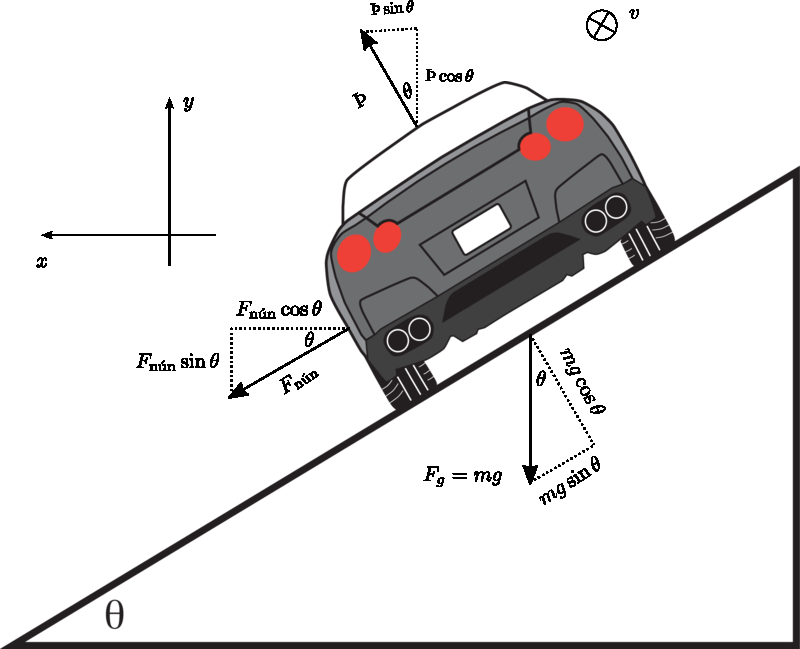
\includegraphics[width=2.7in]{figures/bill.pdf}
\caption{Bíll keyrir með hraða $v$ í NASCAR beygju.}
\label{fig:bill}
\end{wrapfigure}

Hvers vegna eru beygjurnar á NASCAR brautunum í halla? Við skulum skoða það aðeins núna.

\begin{align*}
    \vec{F}_{\text{heild}} = \vec{F}_g + \vec{\text{Þ}} + \vec{F}_{\text{nún}}.
\end{align*}
Sem gefur þá miðað við venjulega kartesíska hnitakerfið:

\begin{align*}
    \begin{pmatrix} m a \\ 0 \end{pmatrix} = \begin{pmatrix} \text{Þ}\sin\theta + F_{\text{nún}}\cos\theta \\ \text{Þ}\cos\theta - mg - F_{\text{nún}}\sin\theta \end{pmatrix}
\end{align*}

Við viljum síðan ákvarða stærsta kyrrstöðunúninginn, $F_{nún} \leq \mu_s \text{Þ}$ þannig að bíllinn fari ekki útaf brautinni. Við notum að hluturinn er á hringhreyfingu þannig að $a = \frac{v^2}{r}$ þar sem $v$ er hraði bílsins og $r$ er geisli hjúfurhrings brautarinnar í beygjunni. Áður en hluturinn byrjar að renna er $F_{\text{nún}} = \mu_s \text{Þ}$ svo við fáum úr neðri jöfnunni að:

\begin{align*}
    0 = \text{Þ} \cos\theta - mg - \mu_s \text{Þ} \sin\theta \implies \text{Þ} = \frac{mg}{\cos\theta - \mu_s \sin\theta}
\end{align*}
En með því að stinga inn í efri jöfnuna höfum við að:
\begin{align*}
    m \frac{v^2}{r} = ma = \text{Þ} \sin\theta + \mu_s Þ \cos\theta = \frac{\sin\theta + \mu_s \cos\theta}{\cos\theta - \mu_s \sin\theta} mg
\end{align*}
En það gefur okkur því að hámarkshraðinn í NASCAR beygju er gefinn með:
\begin{align*}
    v = \sqrt{\left(\frac{\sin\theta + \mu_s \cos\theta}{\cos\theta - \mu_s \sin\theta}\right)gr}.
\end{align*}
Við tökum eftir því að þegar $\theta = 0$ þá fáum við að hámarkshraðinn í flatri beygju er $v = \sqrt{\mu_s gr}$. Ef brautin er núningslaus sjáum við að hámarkshraðinn verður $v = \sqrt{\tan(\theta) gr}$. Við sjáum einnig að því stærra sem $\theta$ er því stærri verður hámarkshraðinn í brautinni. En það þýðir að NASCAR ökuþórarnir geta keyrt hraðar í slíkum beygjum. T.d. er dæmigerður kyrrstöðunúningsstuðull milli dekkja og malbiks gefinn með $\mu_s = \SI{0.90}{}$ og dæmigerður geisli hjúfurhrings á NASCAR braut er $r = \SI{225}{m}$ og brautirnar halla yfirleitt um $\theta = \ang{35}$. Ef brautirnar myndu ekki halla væri hámarkshraðinn sem NASCAR ökumaður gæti keyrt með í beygjunum gefinn með $v = \SI{45}{m/s} = \SI{160}{km/klst}$. Hinsvegar, þar sem brautin hallar um $\theta = \ang{35}$ miðað við lárétt, þá er hámarkshraðinn sem NASCAR ökumenn geta keyrt í beygjunum gefinn með $v = \SI{98}{m/s} = \SI{350}{km/klst}$.  

\end{minipage}

\subsection*{Hómer Simpson og dauðahnötturinn}

Í bíómyndinni \duck{The Simpsons Movie} sem kom út árið 2007 tekst Hómer að keyra hring á mótorhjóli í svokölluðum dauðahring. Við skulum skoða minnsta hraðann sem Hómer þarf að hafa til þess að hann detti ekki niður í efstu stöðu. Ef við skrifum þá niður kraftajöfnu í efstu stöðu þá höfum við að:
\begin{align*}
    ma = mg + \text{Þ}
\end{align*}
Þar sem $\text{Þ}$ er þverkrafturinn frá brautinni á Hómer í efstu stöðu. Þar sem að Hómer er á hringhreyfingu þá höfum við að $a = \frac{v^2}{r}$ svo við höfum að:
\begin{align*}
    m \frac{v^2}{r} = mg + \text{Þ}
\end{align*}
Við ályktum því að þverkrafturinn sem að verkar á Hómer frá brautinni í efstu stöðu er gefinn með:
\begin{align*}
    \text{Þ} = m \frac{v^2}{r} - mg
\end{align*}
En ef Hómer hefur ekki nægan hraða í efstu stöðu þá mun hann detta niður. En þá finnur hann ekki fyrir neinum þverkrafti frá brautinni. Svo minnsti hraðinn þannig að hann sleppi hefur þann eiginleika að $\text{Þ} = 0$ en þar með höfum við að:
\begin{align*}
    0 = m \frac{v^2}{r} - mg \implies v = \sqrt{gr}
\end{align*}
Er minnsti hraðinn sem Hómer getur haft í efstu stöðu dauðahringsins án þess að detta niður og hálsbrotna.

\subsection*{Fjarlægð Venusar frá sólinni}

Hugsum okkur að við fylgjumst með því hversu lengi Venus er að fara hringinn í kringum sólina. Við tökum þá eftir því að það tekur Venusi \SI{225}{daga} að fara hringinn í kringum sólina á meðan að það tekur jörðina \SI{365}{daga} að fara hringinn í kringum jörðina. Við ættum kannski að taka fram að hér erum við að tala um jarðardaga þar sem að einn Venusardagur (þ.e.a.s.~tíminn sem það tekur Venusi að snúast um sjálfa sig) eru rúmir \SI{117}{\text{jarðardagar}}. Við segjum þá að Venusarárið sé \SI{225}{dagar}. Við vitum að fjarlægðin milli jarðarinnar og sólarinnar er $a_{_J} = \SI{1}{AU} = \SI{1.5e11}{m}$. Við getum þá notað lögmál Keplers til þess að ákvarða fjarlægðina milli Venusar og sólarinnar. Við höfum nefnilega samkvæmt þriðja lögmáli Keplers að:
\begin{align*}
    \frac{a_{_J}^3}{T_{_J}^2} = \frac{GM_s}{4\pi^2} = \frac{a_{_V}^3}{T_{_{V}}^2}
\end{align*}
Þar sem að $M_s$ er massi sólarinnar. Þarna höfum við notað að þriðja lögmál Keplers gildir bæði fyrir Jörðina og fyrir Venusi þar sem að báðar pláneturnar eru á hringhreyfingu um sólina. En þar með fáum við að:
\begin{align*}
   \frac{a_{_J}^3}{T_{_J}^2} =  \frac{a_{_V}^3}{T_{_V}^2} \implies a_{_V}^3 = \frac{T_{_V}^2}{T_{_J}^2} a_{_{J}}^3 \implies a_{_V} = \left(\frac{T_{_V}}{T_{_J}}\right)^{3/2} a_{_J} = \left( \frac{225}{365} \right)^{3/2} \SI{1}{AU} = \SI{0.72}{AU}.
\end{align*}

\subsection*{Massi jarðarinnar}

Það má líka nota þriðja lögmál Keplers til þess að ákvarða massa jarðarinnar, $M_{_J}$. Fjölmargar rannsóknir hafa verið gerðar til þess að mæla vegalengdina milli jarðarinnar og tunglsins. Ein slík er að skjóta leysigeisla í áttina að jörðinni og taka tímann á því hversu lengi geislinn er að ferðast fram og til baka (hraði ljósins, $c = \SI{3.00e8}{m/s}$ er bæði takmarkaður og fastur). Það tekur ljósið um það bil $\SI{2.5}{s}$ að fara fram og tilbaka. Þannig fæst að vegalengdin milli jarðarinnar og tunglsins er gefin með $a_{_{T}} = \SI{3.84e8}{m}$. Við vitum líka út frá tunglárinu að það tekur tunglið $T_{_{T}} = \SI{27}{daga}$ að fara umhverfis jörðina. En þar með höfum við samkvæmt þriðja lögmálinu að:
\begin{align*}
    \frac{a_{_T}^3}{T_{_{T}}^2} = \frac{GM_{_J}}{4\pi^2}
\end{align*}
En með því að leysa fyrir massann $M_{_J}$ höfum við því að:
\begin{align*}
    M_{_{J}} = \frac{4\pi^2}{G} \frac{a_{_T}^3}{T_{_{T}}^2} = \frac{4\pi^2}{\SI{6.67e-11}{m^3/(kg.s^2)}} \frac{(\SI{3.84e8}{m})^3}{(27 \cdot 24 \cdot 60^2 \si{s})^2} = \SI{6.16e24}{kg}.
\end{align*}
Sem er ekki í fjarri lagi frá viðteknu gildi $M_{_J} = \SI{5.97e24}{kg}$.

\newpage

\section{Dæmi}

\begin{enumerate}[label = \textbf{Dæmi \thechapter.\arabic*.}]

\subsection*{Þyngdarlögmálið}

\item Geisli tunglsins er $\SI{1.74e6}{m}$ og massi tunglsins er $\SI{7.35e22}{kg}$. Hver er þyngdarhröðunin á tunglinu?

\item Geisli plánetunnar Mars er $R = \SI{3390}{km}$ og massi plánetunnar er $M = \SI{6.39e23}{kg}$. Hver er þyngdarhröðunin á Mars?

\item Í Ástardúett Stuðmanna kemur fram að ástin milli Hörpu Sjafnar og Kristins stuðs sé svo sterk að þau séu magnvana og máttlaus. Hversu stór þyngdarlögmálskraftur verkar á milli þeirra ef massi Kristins er $m_K = \SI{88}{kg}$ og massi Hörpu er $\SI{67}{kg}$ og þau (réttara sagt massamiðjur þeirra) eru í fjarlægðinni $r = \SI{8.5}{cm}$ frá hvert öðru? Hver er hröðun Kristins í áttina að Hörpu? En hröðun Hörpu í áttina að Kristni? Hvort þeirra laðast meira að hinu? 

\item Árið 2015 fann NASA fjarreikistjörnuna Kepler-452b en hún hefur stundum verið kölluð frænka jarðarinnar (hvað sem það nú þýðir). Fjarreikistjarnan Kepler-452b er fimm sinnum massameiri heldur en jörðin, þ.e. $M_K = 5M_J$ og geisli hennar er helmingi stærri, þ.e. $R_K = 1.5R_J$. Hver er þyngdarhröðunin á Kepler-452b?

\item Hver er þyngdarlögmálskrafturinn sem verkar á manneskju sem stendur á jörðinni, $F_J$? Hver er þyngdarlögmálkrafturinn, $F_E$, sem verkar á manneskju sem stendur á toppi Everest í $\SI{8848}{m}$ hæð yfir jörðu? Í hvaða hæð yfir jörðu er þyngdarlögmálskrafturinn sem verkar á manneskju aðeins helmingurinn af þyngdarkraftinum sem verkar á manneskju á jörðinni?

\item Meðalfjarlægðin milli jarðarinnar og tunglsins er $d = \SI{384400}{km}$. Massi jarðarinnar er $M_J = \SI{5.97e24}{kg}$ og massi tunglsins er $M_T = \SI{7.35e22}{kg}$. Til er punktur, sem nefnist Lagrange-punktur, á milli jarðarinnar og tunglsins þar sem að þyngdarkrafturinn frá jörðinni er jafn stór og þyngdarkrafturinn frá tunglinu en það þýðir að enginn heildarkraftur verkar á hlut sem er staðsettur þar. Hversu langt frá jörðinni er Lagrange-punkturinn milli jarðarinnar og tunglsins?

\subsection*{Hringhreyfing}

\item Bíll með massa $\SI{1200}{kg}$ keyrir á láréttri, hringlaga, kappakstursbraut með geisla $\SI{90}{m}$. Hver er mesti hraðinn sem að bíllinn getur keyrt með ef að núningsstuðullinn milli bílsins og brautarinnar er $\mu = \SI{0.65}{}$.

\item Davíð ætlar að slöngva steini í höfuðið á Golíat. Hann setur stein með massa $\SI{1}{kg}$ í slöngvuna og byrjar að sveifla henni í hring í láréttu plani. Slöngvan er $\SI{40}{cm}$ á lengd og miðlægur kraftur sem verkar á steininn er $\SI{10}{N}$. Hver er hraði steinsins?

\item Barn með massa $m = \SI{32}{kg}$ situr kyrrt á risastórum disk sem snýst einn hring á $\SI{3.0}{s}$. Barnið situr í fjarlægð $\SI{1.3}{m}$ frá miðju disksins.
\begin{enumerate}[label = \textbf{(\alph*)}]
    \item Teiknið kraftamynd fyrir barnið.
    \item Hver er stærð miðsóknarkraftsins sem verkar á barnið?
\end{enumerate}

\begin{minipage}{\linewidth}
\begin{wrapfigure}{r}{1.5in}
\vspace{-2.5cm}
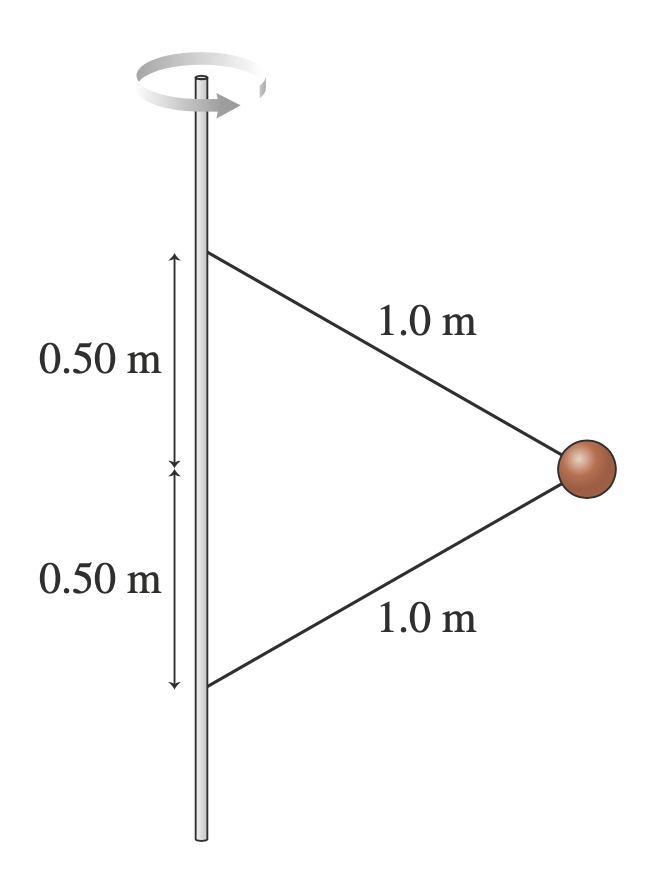
\includegraphics[width=1.5in]{images/hringhreyfing1.png}
\end{wrapfigure}

\item Tveir vírar eru festir við kúlu með massa $m = \SI{300}{g}$. Kúlan er á hringhreyfingu um stöngina með jöfnum hraða $v = \SI{7.5}{m/s}$. Hver er togkrafturinn í vírunum?
\end{minipage}

\vspace{0.25cm}

\begin{minipage}{\linewidth}
\begin{wrapfigure}{r}{1.5in}
\hspace{1.5cm}
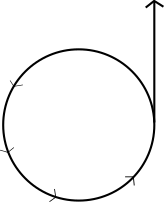
\includegraphics[width=0.8in]{images/parisarhjol.png}
\end{wrapfigure}

\item Parísarhjól með $\SI{20}{m}$ geisla snýr vögnum í hringi, hver með massa $\SI{500}{kg}$. Vagnana ber við jörðu í lægstu stöðu. Dag einn bilar vélbúnaður hjólsins. Það byrjar að snúast of hratt þannig að á hvern vagn verkar $\SI{3000}{N}$ miðsóknarkraftur. Allt í einu losnar vagn af hjólinu með þeim afleiðingum að hann þýtur beint upp á við. Hvaða hæð yfir jörðu nær vagninn áður en hann byrjar að falla aftur til jarðar?

\end{minipage}

\newpage

\begin{minipage}{\linewidth}
\begin{wrapfigure}{r}{1.5in}
\vspace{-1cm}
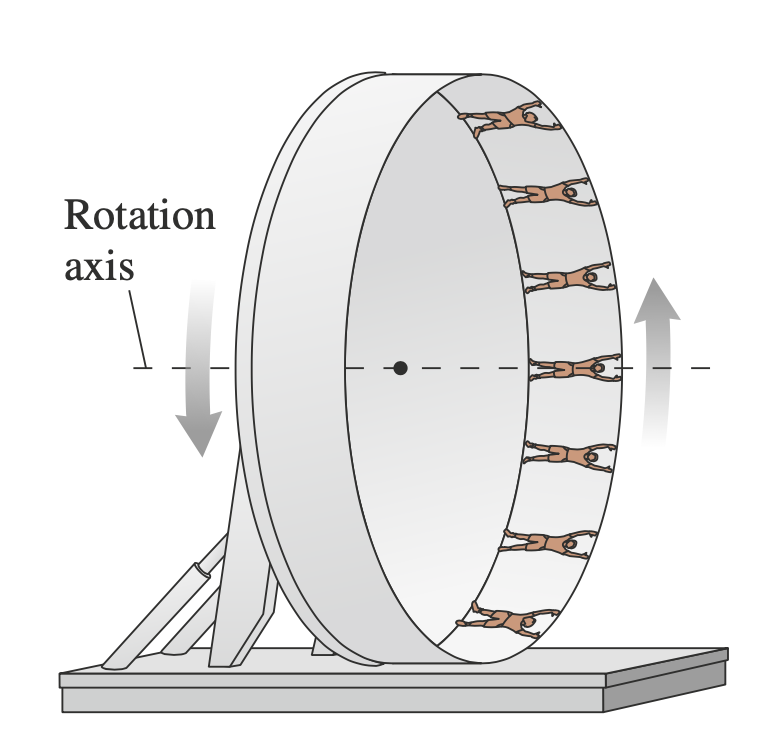
\includegraphics[width=1.5in]{images/hringhreyfing2.png}
\end{wrapfigure}

\item Skemmtigarðurinn í Smáralind var að fjárfesta í nýju tæki sem kallast Hamstrahjólið. Farþegar koma sér fyrir á jaðri hringsins sem hefur geisla $r = \SI{8.0}{m}$. Hringurinn byrjar láréttur en snýst síðan upp í lóðrétta stöðu eins og sjá má á myndinni hér til hægri. Hamstrahjólið snýst einn hring á $\SI{4.5}{s}$ í lóðréttri stöðu. Farþegi með massa $m = \SI{65}{kg}$ fer nú í tækið.

\begin{enumerate}[label = \textbf{(\alph*)}]
    \item Hver er þverkrafturinn sem að farþeginn finnur fyrir í efstu stöðu?
    
    \item Hver er þverkrafturinn sem að farþeginn finnur fyrir í lægstu stöðu?
    
    \item Hver er minnsti umferðartíminn sem að Hamstrahjólið má hafa án þess að farþegarnir falli úr tækinu?
\end{enumerate}

\begin{wrapfigure}{r}{1.5in}
\vspace{-1.5cm}
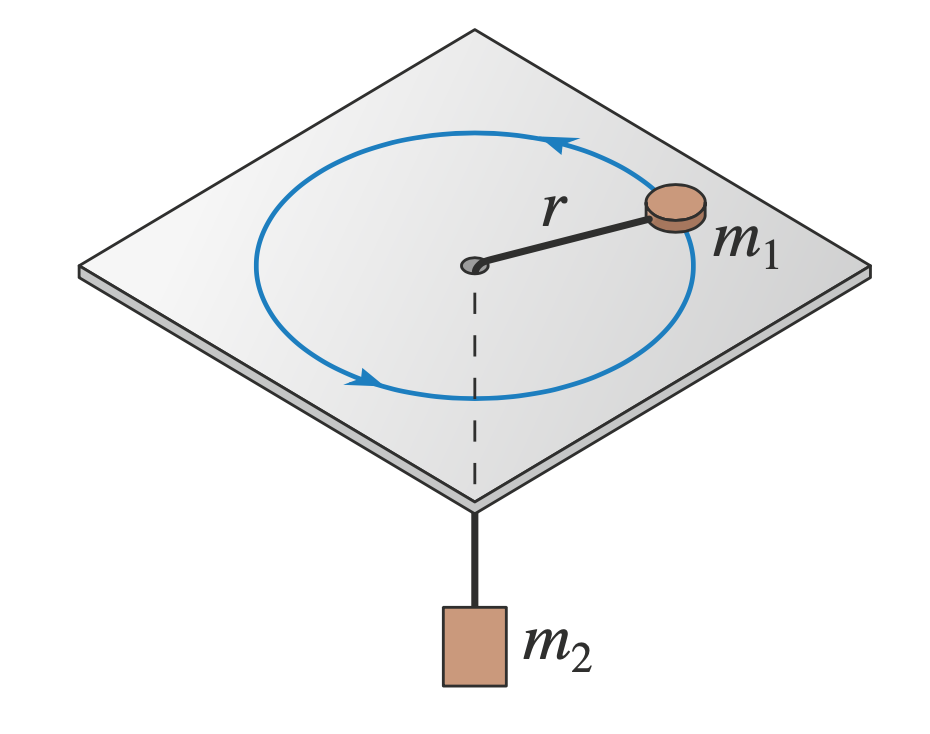
\includegraphics[width=1.5in]{images/hringhreyfing3.png}
\end{wrapfigure}

\item Massi $m_1$ er á hringhreyfingu með geisla $r$ á láréttu, núningslausu borði. Massinn $m_1$ er festur með bandi við massa $m_2$ (það er gat í miðju borðsins) sem hangir lóðrétt undir borðinu. Massinn $m_2$ er kyrr. Hver er hraði $m_1$?
\end{minipage}

\begin{minipage}{\linewidth}
\begin{wrapfigure}{r}{1.5in}
\vspace{-0.5cm}
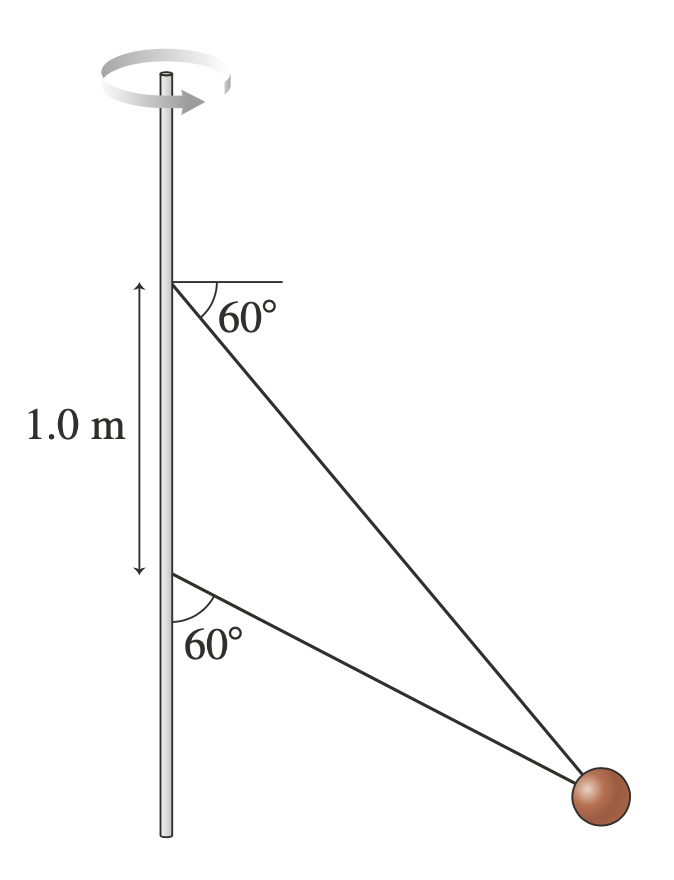
\includegraphics[width=1.5in]{images/hringhreyfing4.png}
\end{wrapfigure}

\item Tveir vírar eru festir við kúlu með massa $m = \SI{2.0}{kg}$ eins og sést á myndinni hér til hægri. Kúlan er á láréttri hringhreyfingu með föstum hraða $v = \SI{2.5}{m/s}$. Hver er togkrafturinn í hvorum vír fyrir sig?

\item Homer Simpson ($\SI{109}{kg}$) ætlar að keyra í hring á mótorhjólinu sínu inni í dauðahnettinum. Þá mun Homer vera á hvolfi efst í hnettinum. Dauðahnötturinn hefur geisla $\SI{20.3}{m}$.
\begin{enumerate}[label = \textbf{(\alph*})]
    \item Hver er minnsti hraðinn sem Hómer þarf að hafa í efstu stöðu þannig að hann falli ekki?
    
    \item Hversu mikill þverkraftur verkar á Homer efst ef hann fer með hraðanum $\SI{80.0}{km/klst}$?
\end{enumerate}

\end{minipage}

\item Festum band með lengd $\ell$ við fötu sem er full af vatni. Látum heildarmassa vatnsins vera $m$. Er hægt að sveifla bandinu heilan hring án þess að vatnið detti úr fötunni?

\item Jójó með massa $\SI{100}{g}$ er sveiflað í bandi í lóðrétta hringi með geisla $\SI{40}{cm}$.
\begin{enumerate}[label = \textbf{(\alph*)}]
    \item Gerið kraftamyndir og kraftajöfnur fyrir jójóið bæði í efstu og neðstu stöðu.
    \item Hver þarf lágmarkshraði jójósins að vera í efstu stöðu svo að ekki slakni á bandinu?
    \item Notið orkuvarðveislu til þess að finna hraða jójósins þegar það er í efstu stöðu ef það hefur hraðann $\SI{5.5}{m/s}$ þegar það er í neðstu stöðu.
    \item Hver er þá togkrafturinn í efstu stöðu?
\end{enumerate}

\subsection*{Lögmál Keplers}

\item Neptúnus er í meðalfjarlægð $\SI{4.5e9}{km}$ frá sólu. Hversu langt er eitt ár á Neptúnusi?

\item Meðalfjarlægð sólarinnar og jarðarinnar er $\SI{1}{AU} = \SI{1.5e11}{m}$. Nýtið ykkur þriðja lögmál Keplers til þess að ákvarða massa sólarinnar.

\item Meðalfjarlægð tunglsins og jarðarinnar er $\SI{384400}{km}$. Nýtið ykkur þriðja lögmál Keplers til þess að ákvarða massa jarðarinnar.

\item Gervihnöttur með massa $\SI{5500}{kg}$ er á sporbraut um jörðina og hefur umferðartíma $\SI{6600}{s}$. Ákvarðið:
\begin{enumerate}[label = \textbf{(\alph*)}]
    \item Geisla sporbrautarinnar.
    \item Stærð þyngdarlögmálkraftsins á gervihnöttinn.
    \item Hæð gervihnattarins yfir jörðu.
\end{enumerate}

\item Mars er fjórða reikistjarnan frá sólu. Mars hefur massa $\SI{6.42e23}{kg}$ og tvö tungl, Fóbos og Deimos. Umferðartími plánetunnar um sólina er $\SI{687}{dagar}$. Mars hefur massa $\SI{6.42e23}{kg}$, geisla $\SI{3390}{km}$. Fóbos er það tungl í sólkerfinu sem er næst reikistjörnu sinni. Fóbos er í $\SI{9380}{km}$ fjarlægð frá miðju Mars. 
\begin{enumerate}[label = \textbf{(\alph*)}]
    \item Hver er þyngdarhröðunin á Mars?
    
    \item Hversu langt frá sólinni er Mars?
    
    \item Hver er umferðartími Fóbosar á sporbraut sinni um Mars?
\end{enumerate}

\item Alþjóðlega geimstöðin er á hringlaga braut umhverfis jörðina $\SI{409}{km}$ frá yfirborði jarðar. Umferðartími hennar er 93 mínútur. Hubble geimsjónaukinn er einnig á hringlaga braut umhverfis jörðina með umferðartíma 96 mínútur. Hve langt frá yfirborði jarðar er Hubble geimsjónaukinn?

\item Árið 2061 mun halastjarna Halleys sjást með berum augum frá jörðinni. Halastjarnan er á sporbraut um sólina og mun ljúka fjórðu umferð sinni um sólu frá því að Edmond Halley spáði fyrir um komu hennar fyrst, árið 1758. Þegar halastjarnan var síðast í nándarstöðu, árið 1986 mældist hún í fjarlægðinni $r_p = \SI{0.59}{AU}$ frá sólu. Hver er mesta fjarlægðin, $r_a$, sem að halastjarna Halleys nær í firrðarstöðu, frá sólu?

\item Venus er önnur reikistjarnan frá sól. Af öllum reikistjörnum í sólkerfinu er braut Venusar sú sem kemst næst því að vera hringlaga. Reikistjarnan lýkur einni hringferð um sólina á $245$ jarðardögum. Jörðin ferðast með hraðanum $\SI{30}{km/s}$ um sólina. Hver er hraði Venusar?

\item Dvergreikistjarnan Plútó gengur um sólu á sporöskjulaga braut. Mesta fjarlægð hennar frá sólu er $\SI{49.3}{AU}$ og minnsta fjarlægð hennar frá sólu er $\SI{29.7}{AU}$. Hver er umferðartími Plútó?


\item Braut Venusar um sólina er næstum hringlaga. Venus er í $\SI{0.72}{AU}$ fjarlægð frá sólu. ($\SI{1}{AU} = \SI{1.5e11}{m}$). Notið þriðja lögmál Keplers til að finna umferðartíma Venusar.

\item Sporbaugur stærsta tungls Júpiters, Ganymede, um plánetuna er nærri því hringlaga með geisla $\SI{1.07e6}{km}$. Umferðartími Ganymede er $\SI{7.16}{dagar}$. Hver er massi Júpíters?

\end{enumerate}


\section*{Svör}

\begin{enumerate*}[label = \vspace{0.15cm} \textbf{(\arabic*)}]
  \item $g_{_T} = \SI{1.62}{m/s^2}$.
  \item $g_{_M} = \SI{3.71}{m/s^2}$.
  \item $F_G = \SI{54}{\mu N}$, $a_{_K} = \SI{6.1e-7}{m/s^2}$, $a_{_H} = \SI{8.1e-7}{m/s^2}$, Harpa.
  \item $g_{_K} = \SI{21.8}{m/s^2}$.
  \item $F_J = \frac{GmM_J}{R_J^2}$, $F_E = \frac{Gm M_J}{(R_j + h)^2}$,  $h = \SI{2640}{km}$.
  \item $x = \SI{346000}{km}$.
  \item $\SI{24}{m/s}$.
  \item $\SI{2}{m/s}$.
  \item $\SI{185}{N}$.
  \item $T_1 = \SI{14}{N}$, $T_2 = \SI{8.3}{N}$.
  \item $h_{\text{max}} = \SI{26}{m}$.
  \item $Þ = \SI{380}{N}$, $Þ = \SI{1660}{N}$, $T= \SI{5.6}{s}$.
  \item $v = \sqrt{\frac{m_2}{m_1}gr}$.
  \item $T_1 = \SI{15}{N}$, $T_2 = \SI{7.9}{N}$.
  \item $v_{\text{min}} = \SI{14.1}{m/s}$, $Þ = \SI{1580}{N}$.
  \item $v > \sqrt{gl}$.
  \item $v = \SI{2.0}{m/s}$, $v = \SI{3.8}{m/s}$, $Þ = \SI{2.6}{N}$.
  \item $T_{_N} = \SI{164}{ár}$.
  \item $M_{_S} = \SI{2.0e30}{kg}$.
  \item $M_{_J} = \SI{5.7e24}{kg}$.
  \item $a = \SI{7134}{km}$, $F_G = \SI{43000}{N}$, $h = \SI{763}{km}$.
  \item $g_{_M} = \SI{3.62}{m/s^2}$, $a_{_M} = \SI{1.52}{AU}$, $T_{_F} = \SI{7}{klst}$ og $\SI{40}{mín}$.
  \item $h_{_H} = \SI{545}{km}$.
  \item $r_{\text{max}} = \SI{35.2}{AU}$.
  \item $v = \SI{34}{km/s}$.
  \item $T_{_P} = \SI{248}{ár}$.
  \item $T_{_V} = \SI{223}{dagar}$.
  \item $M_{_J} = \SI{1.89e27}{kg}$.
\end{enumerate*}

\newpage